\documentclass[10pt,aspectratio=169]{beamer}

\usetheme[sectionpage=simple,numbering=fraction]{metropolis}
\usepackage{appendixnumberbeamer}

\usepackage{booktabs}
\usepackage[scale=2]{ccicons}

\usepackage{pgfplots}
\usepgfplotslibrary{dateplot}

\usepackage{xspace}
\newcommand{\themename}{\textbf{\textsc{metropolis}}\xspace}

\title{\hspace{\linewidth}\\Introduction to parallisation in OpenFOAM}
\date{June 02, 2022}
\author{Mohammed Elwardi Fadeli\textsuperscript{1,2}, Holger Marschall\textsuperscript{1} and Christian Hasse\textsuperscript{2}}
\institute{
    \textsuperscript{1} Mathematical Modeling and Analysis (MMA)\\
    \textsuperscript{2} Simulation of Reactive Thermo Fluid Systems (STFS)\\
        TU Darmstadt
}
% \titlegraphic{\hfill\includegraphics[height=1.5cm]{logo.pdf}}

\definecolor{mDarkBrown}{HTML}{604c38}
\definecolor{mDarkTeal}{HTML}{0F1833}
\definecolor{mLightBrown}{HTML}{EB811B}
\definecolor{mLightGreen}{HTML}{14B03D}
\colorlet{mBg}{black!2}

\usepackage{amsmath, amsfonts}
\usepackage{multicol}
\usepackage{tikz-3dplot}
\usetikzlibrary{arrows.meta, calc, tikzmark, shapes.geometric, positioning, automata}
\usepackage{setspace}
\usepackage{stmaryrd}
\usepackage[most]{tcolorbox}
\tcbuselibrary{listings}
\tcbuselibrary{minted}
\usepackage{pgfplots}

\newenvironment{CodeEnv}[4][]
{\tcbset{mytcboptions/.style={title=#1}}%
    \tcblisting{
    listing only,width=\linewidth,colback=white,colframe=mDarkTeal,
    arc=0pt,outer arc=0pt,top=1mm,bottom=1mm,left=1mm,right=1mm,
    listing outside comment,righthand width=2.5cm,comment={#3},
    boxrule=0.6pt,listing engine=minted,minted language=#2,mytcboptions,minted options={fontsize=#4,escapeinside=??}%
}
}{%
\endtcblisting%
}

\newenvironment{CodeEnvNoComment}[3][]
{\tcbset{mytcboptions/.style={title=#1}}%
    \tcblisting{
    listing only,width=\linewidth,colback=white,colframe=mDarkTeal,
    arc=0pt,outer arc=0pt,top=1mm,bottom=1mm,left=1mm,right=1mm,
    boxrule=0.6pt,listing engine=minted,minted language=#2,mytcboptions,minted options={fontsize=#3,escapeinside=??}%
}
}{%
\endtcblisting%
}


\tikzset{
  loris1/.style={
    path picture={
      \node[anchor=center] at (path picture bounding box.center) {
        \includegraphics[scale=.5]{images/slow_loris.jpg}};}},
  loris2/.style={
    path picture={
      \node[anchor=center] at (path picture bounding box.center) {
        \includegraphics[scale=.5]{images/slow_loris_blueish.png}};}},
  process/.style={
  rectangle, minimum width=1cm, minimum height=1cm, thick, draw = white, node distance = 26mm},
  note/.style={
    fill=mLightGreen, draw=mLightGreen, inner sep=0.1cm, anchor=east, text=white
  },
  lownote/.style={
    fill=mDarkBrown, draw=mDarkBrown, inner sep=0.1cm, anchor=west,text=white
  }
}
\tikzstyle{noteNode} = [fill=my_yellow, draw=my_yellow, inner sep=0.1cm, anchor=east]

\newcommand{\DrawBox}[5]{% lx, ly, dx, dy, dz
        \def\lx{#1}
        \def\ly{#2}
        \def\dx{#3}
        \def\dy{#4}
        \def\dxplx{\lx+\dx}
        \def\offset{.25}
        \def\dyply{\ly+\dy}
        \draw[cube,fill=black!2] (\dx,\dy,#5) -- (\dx,\dyply,#5) -- (\dxplx,\dyply,#5) -- (\dxplx,\dy,#5) -- cycle;
        \draw[cube,fill=black!2] (\dxplx,\dy,#5) -- (\dxplx,\dy,0) -- (\dxplx,\dyply,0) -- (\dxplx,\dyply,#5) -- cycle;
        \draw[cube,fill=black!2] (\dxplx,\dyply,#5) -- (\dxplx,\dyply,0) -- (\dx,\dyply,0) -- (\dx,\dyply,#5) -- cycle;
        \pgfmathsetmacro{\xlo}{\dx+\offset}
        \pgfmathsetmacro{\xfs}{\dx+\offset+\offset}
        \pgfmathsetmacro{\xhi}{\lx+\dx}
        \pgfmathsetmacro{\ylo}{\dy+\offset}
        \pgfmathsetmacro{\yfs}{\dy+\offset+\offset}
        \pgfmathsetmacro{\yhi}{\ly+\dy}
        \foreach \x in {\xlo,\xfs,...,\xhi}
        	\foreach \y in {\ylo,\yfs,...,\yhi}
        	{
        		\draw[grid] (\x,\dy,#5) -- (\x,\yhi,#5);
        		\draw[grid] (\dx,\y,#5) -- (\xhi,\y,#5);
        	}

        \foreach \x in {\xlo,\xfs,...,\xhi}
        	\foreach \z in {0.25,0.5,...,1.75}
        	{
        		\draw[grid] (\x,\yhi,0) -- (\x,\yhi,2);
        		\draw[grid] (\dx,\yhi,\z) -- (\xhi,\yhi,\z);
        	}

        \foreach \y in {\ylo,\yfs,...,\yhi}
        	\foreach \z in {0.25,0.5,...,1.75}
        	{
        		\draw[grid] (\xhi,\y,0) -- (\xhi,\y,2);
        		\draw[grid] (\xhi,\dy,\z) -- (\xhi,\yhi,\z);
        	}

}

\titlegraphic{\begin{flushright}\includegraphics[width=.45\textwidth]{images/nhr-tu-logo.png}\end{flushright}}
\setbeamerfont{page number in head/foot}{size=\tiny}
\setbeamercolor{footline}{fg=gray}
\setbeamertemplate{frame footer}{Supported by NH4CES}

\usepackage[doi=true,style=numeric]{biblatex}
  \nocite{*}
  \setbeamertemplate{bibliography item}[text]
  \addbibresource{openfoam-parallelisation.bib}

\setlength{\abovecaptionskip}{2pt}

\begin{document}

\maketitle

\begin{frame}{Table of contents}
  \setbeamertemplate{section in toc}[sections numbered]
  \tableofcontents[hideallsubsections]
\end{frame}

\section{Introduction}

\begin{frame}<1>[fragile,label=f1]
    \frametitle<1>{The power of parallel workers}
    \frametitle<2>{P2P comms: A first example}
    \frametitle<3>{Oh, there is a reduce here!}
    \frametitle<4>{What if one of them just walks away mid-op?}
    \begin{figure}
        \begin{center}
        \begin{tikzpicture}
            \node[anchor=south west,inner sep=0] at (0,0) {\includegraphics[height=0.7\pageheight]{images/Ferrari_pit_stop.jpg}};
            \draw<2>[mLightGreen,ultra thick,fill=mLightGreen,fill opacity=.2] (4.5,5) rectangle (6,6);
            \draw<2>[mLightGreen,ultra thick,fill=mLightGreen,fill opacity=.2] (5,3.5) rectangle (6.5,4.5);

            \draw<3>[mLightBrown,ultra thick,fill=mLightBrown,fill opacity=.2] (7,5) rectangle (8,6);
            \draw<3>[mLightGreen,ultra thick,fill=mLightGreen,fill opacity=.2] (4,3) rectangle (5,4);
            \draw<3>[mLightGreen,ultra thick,fill=mLightGreen,fill opacity=.2] (7,3.5) rectangle (8,4.5);
            \draw<3>[mLightGreen,ultra thick,fill=mLightGreen,fill opacity=.2] (5.9,4.8) rectangle (6.9,5.8);
        \end{tikzpicture}
        \end{center}
        \caption{Parallel work during F1 Pit stops;  \tiny CC BY 2.0, from commons.wikimedia.org}
        \label{fig:}
    \end{figure}
\end{frame}

\begin{frame}[fragile]{Types of Parallelism}
    \setbeamercovered{transparent}
    \begin{description}
        \item[Data Parallelism  \hspace{0.4cm}] \hspace{\linewidth} Work units execute the same operations on a (distributed) set of data: {\bf domain decomposition}.
        \pause
        \item[\alert{Task Parallelism} \hspace{0.4cm}] \hspace{\linewidth} Work units execute on different control paths, possibly on different data sets: {\bf multi-threading}.
        \item[\alert{Pipeline Parallelism}] \hspace{\linewidth} Work split between producer and consumer units that are directly connected. each unit executes a single
            phase of a given task and hands over control to the next one.
    \end{description}
\end{frame}


\begin{frame}[fragile]{Domain decomposition in OpenFOAM}
\begin{description}
    \item[simple\hspace{2cm}] \hspace{\linewidth} 
        Simple geometric decomposition, in which the domain is split into pieces by direction
    \item[hierarchical\hspace{2cm}] \hspace{\linewidth} 
        Same as simple, but the order in which the directional split is done can be specified
    \item[metis \& scotch\hspace{2cm}] \hspace{\linewidth} 
        Require no geometric input from the user and attempts to minimize the number of processor boundaries.
        Weighting for the decomposition between processors can be specified
    \item[manual\hspace{2cm}] \hspace{\linewidth} 
        Allocation of each cell to a particular processor is specified directly.
\end{description}
\end{frame}


\begin{frame}[fragile]{Domain decomposition in OpenFOAM: Processor boundaries}
\begin{figure}
        \tdplotsetmaincoords{60}{125}
    \begin{tikzpicture}
        	[tdplot_main_coords,
        		cube/.style={very thick,black},
        		grid/.style={very thin,gray},
        		axis/.style={->,blue,thick}]
        
        % global mesh
        \DrawBox{2}{2}{0}{0}{2}
        \draw[cube,draw=mLightGreen] (2,1.5,0) -- (2,1.5,2) -- (1.5,1.5,2);
        \draw[cube,draw=mLightGreen] (0,1,2) -- (1.5,1,2);
        \draw[cube,draw=mLightGreen] (1.5,2,0) -- (1.5,2,2) -- (1.5,0,2);
        \node[inner sep=0.1mm] (b0) at (2.5,0,2) {$\Omega_0$};
        \node[inner sep=0.1mm] (b1) at (0,0,2.3) {$\Omega_1$};
        \node[inner sep=0.1mm] (b2) at (0,2,2.3) {$\Omega_2$};
        \node[inner sep=0.1mm] (b3) at (2,2.5,0) {$\Omega_2$};
        
        \path [-stealth] (b0.south) edge [bend left=-20, draw=mDarkTeal,thick] (2,1,1);
        \path [-stealth] (b1) edge [bend left=-20, draw=mDarkTeal,thick] (1.25,.5,2);
        \path [-stealth] (b2) edge [bend left=-20, draw=mDarkTeal,thick] (0.75,1.5,2);
        \path [-stealth] (b3) edge [bend left=-20, draw=mDarkTeal,thick] (1.5,1.75,1);

    \begin{scope}[xshift=5.5cm]
        \DrawBox{1.75}{1.25}{0}{0}{2}
        \draw[fill=gray!20, fill opacity=.8] (\xhi,0,2) -- (\xhi,\yhi,2)  -- (0,\yhi,2) -- (0,\yhi-.25,2)  -- (\xhi-.25,\yhi-.25,2) -- (\xhi-.25,0,2) -- cycle;
        \draw[fill=gray!20, fill opacity=.8] (\xhi,0,2) -- (\xhi,\yhi,2)  -- (0,\yhi,2) -- (0,\yhi,0)  -- (\xhi,\yhi,0) -- (\xhi,0,0)   -- cycle;
        \draw[cube,draw=mLightGreen] (0,1,2) -- (1.5,1,2) -- (1.5,0,2);

        \DrawBox{0.75}{1.75}{2.25}{0}{2}
        \draw[fill=gray!20, fill opacity=.8]  (\dx+.25,0,2) -- (\dx+.25,\yhi-.25,2) -- (\xhi,\yhi-.25,2) -- (\xhi,\yhi-.25,0) -- (\xhi,\yhi,0) 
                                          -- (\dx,\yhi,0) -- (\dx,\yhi,2) --  (\dx,0,2) -- cycle;
        \draw[cube,draw=mLightGreen] (\dx+.25,0,2) -- (\dx+.25,\yhi-.25,2) -- (\xhi,\yhi-.25,2) -- (\xhi,\yhi-.25,0);

        \DrawBox{1.75}{1.25}{0}{1.75}{2}
        \draw[fill=gray!20, fill opacity=.8] (\dx,\dy+.25,2) -- (\xhi-.25,\dy+.25,2) -- (\xhi-.25,\yhi,2) -- (\xhi-.25,\yhi,0)
                                          -- (\xhi,\yhi,0) -- (\xhi,\dy,0)  -- (\xhi,\dy,2) --  (\dx,\dy,2) -- cycle; 
        \draw[cube,draw=mLightGreen] (\dx,\dy+.25,2) -- (\xhi-.25,\dy+.25,2) -- (\xhi-.25,\yhi,2) -- (\xhi-.25,\yhi,0);


        \DrawBox{0.75}{0.75}{2.25}{2.25}{2}
        \draw[fill=gray!20, fill opacity=.8] (\dx+.25,\yhi,0) -- (\dx+.25,\yhi,2) --  (\dx+.25,\dy+.25,2) -- (\xhi,\dy+.25,2) -- (\xhi,\dy+.25,0)
                                          -- (\xhi,\dy,0) -- (\xhi,\dy,2) -- (\dx,\dy,2)  -- (\dx,\yhi,2) -- (\dx,\yhi,0) -- cycle;
        \draw[cube,draw=mLightGreen] (\dx+.25,\yhi,0) -- (\dx+.25,\yhi,2) --  (\dx+.25,\dy+.25,2) -- (\xhi,\dy+.25,2) -- (\xhi,\dy+.25,0);

        \node[inner sep=0.1mm,mLightGreen] (b01) at (2.5,0,2.4) {$\Gamma_0^1$};
        \node[inner sep=0.1mm,mLightGreen] (b10) at (2,0,2.5) {$\Gamma_1^0$};
        \node[inner sep=0.3mm, align=center] (c01) at (3.5,-1,1.4) {\scriptsize\baselineskip=1pt adjoint: $\overline{\phi_0}${\tt +=}$\overline{\phi_1}$\\\baselineskip=1pt  \scriptsize $\overline{\phi_1}=0$};
        \node[inner sep=0.3mm, align=center] (c10) at (3,-1,3.5) {\scriptsize\baselineskip=1pt 0 sends $\phi$,  \scriptsize $\phi_1=\phi_0$};
        \draw[dashed,-stealth] (b01) -- (c01);
        \draw[dashed,-stealth] (b10) -- (c10.south east);
    \end{scope}
    \end{tikzpicture}
    \caption{Classical halo approach for inter-processor communication}
\end{figure}
    
    \begin{itemize}
        \item Use of a layer of ghost cells  to handle comms with neighboring processes $\rightarrow$ MPI calls not self-adjoint
        \item Artificial increase in number of computations per process (and does not scale well)
    \end{itemize}
\end{frame}

\begin{frame}[fragile]{Domain decomposition in OpenFOAM: Processor boundaries}
\begin{figure}
        \tdplotsetmaincoords{60}{125}
    \begin{tikzpicture}
        	[tdplot_main_coords,
        		cube/.style={very thick,black},
        		grid/.style={very thin,gray},
        		axis/.style={->,blue,thick}]
        
        % global mesh
        \DrawBox{2}{2}{0}{0}{2}
        \draw[cube,draw=mLightGreen] (2,1.5,0) -- (2,1.5,2) -- (1.5,1.5,2);
        \draw[cube,draw=mLightGreen] (0,1,2) -- (1.5,1,2);
        \draw[cube,draw=mLightGreen] (1.5,2,0) -- (1.5,2,2) -- (1.5,0,2);
        \node[inner sep=0.1mm] (b0) at (2.5,0,2) {$\Omega_0$};
        \node[inner sep=0.1mm] (b1) at (0,0,2.3) {$\Omega_1$};
        \node[inner sep=0.1mm] (b2) at (0,2,2.3) {$\Omega_2$};
        \node[inner sep=0.1mm] (b3) at (2,2.5,0) {$\Omega_2$};
        
        \path [-stealth] (b0.south) edge [bend left=-20, draw=mDarkTeal,thick] (2,1,1);
        \path [-stealth] (b1) edge [bend left=-20, draw=mDarkTeal,thick] (1.25,.5,2);
        \path [-stealth] (b2) edge [bend left=-20, draw=mDarkTeal,thick] (0.75,1.5,2);
        \path [-stealth] (b3) edge [bend left=-20, draw=mDarkTeal,thick] (1.5,1.75,1);

    \begin{scope}[xshift=5.5cm]
        \DrawBox{1.5}{1}{0}{0}{2}
        \draw[fill=mLightGreen!40,fill opacity=0.6] (0,1,2) -- (1.5,1,2) -- (1.5,0,2) -- (1.5,0,0) -- (1.5,1,0) -- (0,1,0) -- cycle;
        \draw[cube,draw=mLightGreen] (0,1,2) -- (1.5,1,2) -- (1.5,0,2)  (1.5,1,2) -- (1.5,1,0);

        \DrawBox{0.5}{1.5}{2.5}{0}{2}
        \draw[cube,draw=mLightGreen,fill=mLightGreen!40,fill opacity=0.6] (\dx,0,2) -- (\dx,\yhi,2) -- (\xhi,\yhi,2) -- (\xhi,\yhi,0) -- (\dx,\yhi,0) -- (\dx,\yhi,2);

        \DrawBox{1.5}{1}{0}{2}{2}
        \draw[cube,draw=mLightGreen,fill=mLightGreen!40,fill opacity=0.6] (\dx,\dy,2) -- (\xhi,\dy,2) -- (\xhi,\yhi,2) -- (\xhi,\yhi,0)  -- (\xhi,\dy,0) -- (\xhi,\dy,2);


        \DrawBox{0.5}{0.5}{2.5}{2.5}{2}
        \draw[cube,draw=mLightGreen] (\dx,\yhi,0) -- (\dx,\yhi,2) --  (\dx,\dy,2) -- (\xhi,\dy,2) -- (\xhi,\dy,0);

        \node[inner sep=0.3mm,mLightGreen] (b01) at (2.5,0,2.4) {$\Gamma_{0,1}$};
        %\node[inner sep=0.1mm,mLightGreen] (b10) at (2,0,2.5) {$\Gamma_1^0$};
        \node[inner sep=0.3mm, align=center] (c10) at (3,-1,3.5) {\scriptsize cyclic + comms};
        \draw[dashed,-stealth] (b01) -- (c10);
        %\draw[dashed,-stealth] (b10) -- (c10.south east);
    \end{scope}
    \end{tikzpicture}
    \caption{Zero-halo approach for inter-processor communication in OpenFOAM}
\end{figure}
    \begin{itemize}
        \item Communications accross process boundaries handled as a BC
        \item MPI calls are self-adjoint; all processes perform the same work at the boundaries
    \end{itemize}
\end{frame}

\begin{frame}[fragile]{Modes of Parallelism}
    \begin{description}
        \item[Distributed Memory] \hspace{\linewidth} Message Passing Interface ({\bf MPI}): Execute on multiple machines.
        \item[Shared Memory] \hspace{\linewidth} Multi-threading capabilities of programming languages, OpenMP.
        \item[Data Streaming] \hspace{\linewidth} CUDA and OpenCL. Applications are organized into streams (of same-type elements) 
            and kernels (which act on elements of streams).
    \end{description}
\end{frame}


\begin{frame}[fragile]{MPI with OpenFOAM}
\begin{CodeEnv}[Is echo MPI-ready?]{bash}{\tiny Hello World!\\Hello World!\\Hello World!}{\scriptsize}
mpirun -n 3 echo Hello World!
\end{CodeEnv}
    
\begin{CodeEnv}[What about a solver binary?]{bash}{\tiny This runs on "undecomposed" cases!}{\scriptsize}
mpirun -n 3 icoFoam
\end{CodeEnv}

\pause
    
\begin{CodeEnv}[But the solver is linked to libmpi!]{bash}{\tiny ... libmpi.so ...}{\scriptsize}
ldd $(which icoFoam)
\end{CodeEnv}
    
\pause

\begin{CodeEnv}[Alright we get it now]{bash}{\tiny Needs a decomposed case}{\scriptsize}
mpirun -n 3 icoFoam -parallel
\end{CodeEnv}
\end{frame}

\begin{frame}[fragile]{MPI with OpenFOAM: Parallel mode}
    \begin{multicols}{2}
\begin{CodeEnvNoComment}[Anatomy of MPI programs]{cpp}{\tiny}
#include <mpi.h>
void main (int argc, char *argv[])
{
  int np, rank, err;
  err = ?\colorbox{mLightGreen!20}{MPI\_Init(&argc, &argv)}?; 
  MPI_Comm_rank(MPI_COMM_WORLD,&rank);
  MPI_Comm_size(MPI_COMM_WORLD,&np);
  // Do parallel communications
  err = ?\colorbox{mLightGreen!20}{MPI\_Finalize()}?;
}
\end{CodeEnvNoComment}
\columnbreak
\pause
\begin{CodeEnvNoComment}[How solver programs look]{cpp}{\tiny}
#include "fvCFD.H"
void main (int argc, char *argv[])
{
  #include ?\colorbox{mLightGreen!20}{"setRootCase.H"}?
  // Defines an argList object,
  // which has a ParRunControl member
  // If -parallel is passed in:
  // MPI_Init called in its ctor
  // MPI_Finalize called in its dtor

  // Time is constructed with
  // <case>/processor<procID> paths
}
\end{CodeEnvNoComment}
    \end{multicols}

You don't have to know MPI API to parallelise OpenFOAM code!
But you need the concepts.
\end{frame}

\begin{frame}[fragile]{Objectives}
    \begin{enumerate}
        \item Have a basic understanding of Parallel programming with MPI in OpenFOAM Code.
        \item Be able to send basic custom classes around using MPI.
        \item Be aware of some of the common issues around MPI comms.
        \item Aquire enough knowledge  to learn more on your own
        \begin{itemize}
            \item Directly from OpenFOAM's code
            \item MPI in general
        \end{itemize}
    \end{enumerate}
\end{frame}

\begin{frame}[fragile]{Communication types in MPI}

\begin{figure}
    \begin{center}
    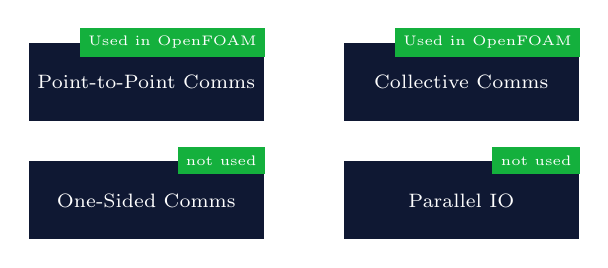
\begin{tikzpicture}
        \node[minimum height=1cm, minimum width=3cm,draw=white, text=white,fill=mDarkTeal] (m0) {\scriptsize Point-to-Point Comms};
        \node[note] (n0) at (m0.north east)  {\tiny Used in OpenFOAM};
        \node[minimum height=1cm, minimum width=3cm,draw=white, text=white,fill=mDarkTeal] (m1) at ($(m0)+(4cm,0)$) {\scriptsize Collective Comms};
        \node[note] (n1) at (m1.north east)  {\tiny Used in OpenFOAM};
        \node[minimum height=1cm, minimum width=3cm,draw=white, text=white,fill=mDarkTeal] (m2) at ($(m0)+(0,-1.5cm)$) {\scriptsize One-Sided Comms};
        \node[note] (n2) at (m2.north east)  {\tiny not used};
        \node[minimum height=1cm, minimum width=3cm,draw=white, text=white,fill=mDarkTeal] (m3) at ($(m1)+(0,-1.5cm)$) {\scriptsize Parallel IO};
        \node[note] (n3) at (m3.north east)  {\tiny not used};
    \end{tikzpicture}
    \end{center}
\end{figure}

\begin{center}
We'll be focusing on the communications OpenFOAM wraps!
\end{center}
\end{frame}

\section{Point-to-Point communication}

\begin{frame}[fragile]{Communicators and ranks}
    There may be many processes talking!
    \begin{description}
        \item[MPI Communicators] \hspace{\linewidth} Objects defining which processes can communicate;
            Processes are refered to by  their {\bf ranks}
        \begin{itemize}
            \item \verb|MPI_COMM_FOAM| in the Foundation version and Foam Extend 5
            \item \verb|MPI_COMM_WORLD| (All processes) elsewhere
            \item Size: \verb|Pstream::nProcs()|
        \end{itemize}
    \item[MPI rank \hspace{1.9cm}] \hspace{\linewidth} Process Identifier (an integer).
        \begin{itemize}
            \item \verb|Pstream::myProcNo()| returns the active process's ID.
        \end{itemize}
    \end{description}
\end{frame}


\begin{frame}[fragile]{P2P comms}

\begin{itemize}
    \item MPI defines its own {\bf Data Types}
    \item OpenFOAM gets around it using {\bf parallel streams}
        \begin{itemize}
            \item OpenFOAM hands over a stream-representation of your data to MPI calls
            \item MPI passes the information in those streams around
        \end{itemize}
\end{itemize}

\begin{figure}
    \begin{center}
    \begin{tikzpicture}
    \node[loris1, process] (p0) [label=above:{\scriptsize $P_0$}] {};
    \node[loris2, process] (p1) at (6,0) [label=above:{\scriptsize $P_1$}] {};
    \node (c) at ($(p0)+(3,-1)$) {   };
    \draw[thick,draw=mDarkTeal,Tee Barb-] (p0) |- (c.west) node [near end,above, mDarkTeal] {\tt OPstream};
    \draw[thick,draw=mLightGreen,-stealth] (c.east) -| (p1) node [near start,above,mLightGreen] {\tt IPstream};

    %\node[node, image] (x_src_i) [right=of y_src_i, label=below:$\phi_j$] { };
    \node (s1) at (3,-1) [semicircle, fill=mLightGreen, minimum size=1mm, rotate=-135, node distance=0,anchor=south] {};
    \node (s1) at (3,-1) [semicircle, fill=mDarkTeal, minimum size=1mm, rotate=45,node distance=0,anchor=south] {};
    \node[draw=mDarkTeal] (b0) at (s1.south) [mDarkTeal,left=.45cm,label=left:{\scriptsize send},rotate=90] {\scriptsize MPI buf};
    \node[draw=mLightGreen] (b1) at (s1.south) [mLightGreen, right=.45cm,label=right:{\scriptsize recv},rotate=-90] {\scriptsize MPI buf};
    \end{tikzpicture}
    \end{center}
    \caption{Communication between two processes in OpenFOAM}
    \label{fig:}
\end{figure}

\end{frame}

\againframe<2>{f1}

\begin{frame}[fragile]{P2P comms: A first example}

    \begin{itemize}
        \item {\tt Pstream} class provides the interface needed for communication
        \item Each "send" must be matched with a "recieve"
    \end{itemize}
\begin{CodeEnvNoComment}[Slaves talk to master]{cpp}{\tiny}
if (Pstream::master())
{
    // Receive lst on master
    for
    (
        int slave=Pstream::firstSlave();
        slave<=Pstream::lastSlave();
        slave++
    )
    {
        labelList lst;
        ?\colorbox{mLightGreen!20}{IPstream fromSlave}?(Pstream::commsTypes::blocking, slave);
        fromSlave >> lst; // Then do something with lst
    }
} else {
    // Send lst to master
    ?\colorbox{mLightGreen!20}{OPstream toMaster}?(Pstream::commsTypes::blocking, Pstream::masterNo());
    toMaster << localLst;
}
\end{CodeEnvNoComment}
\end{frame}

\begin{frame}[fragile]{P2P Blocking comms}

    {\tt Pstream::commsTypes::blocking} (or just {\tt Pstream::blocking} in Foam Extend) defines properties for the MPI call which is executed by
    the constructed stream.
    \begin{itemize}
        \item Does a "local blocking send", i.e. acts on a local buffer
        \item No matching receive available yet? Block until the message is copied into the buffer
        \item Returns when the send buffer is safe to be reused.
        \item Blocking recieve only returns when the receive buffer has the expected data.
        \item Use this if you want to be on the safe side.
        \item But, It may result in deadlocks
    \end{itemize}
\end{frame}

\begin{frame}[fragile]{P2P Blocking comms}

    {\tt Pstream::commsTypes::scheduled} (or just {\tt Pstream::scheduled} in Foam Extend) lets MPI pick the best course of action
    (in terms of performance and memory). This may also depend on the MPI implementation.
    \begin{itemize}
        \item Does a "standard send", Either:
            \begin{enumerate}
                \item The message is directly put in the recieve buffer.
                \item Data is buffered (similar to `blocking`).
                \item Block until a receive shows up.
            \end{enumerate}
        \item Has higher chances of causing deadllocks
    \end{itemize}

    \begin{description}
        \item[A Deadlock] happens when a process is waiting for a message that never reaches it.
    \end{description}
\end{frame}



\begin{frame}[fragile]{P2P Blocking comms: Deadlocks}

    \begin{itemize}
        \item Either a matching send or a recieve is missing (Definitely a deadlock).
        \item A send-recieve cycle (Incorrect usage or order of send/recieve calls).
    \end{itemize}
\begin{figure}

    \begin{center}
    \begin{tikzpicture}
    \node[loris1, process] (p0) [label=above:{\scriptsize $P_0$}] {};
    \node[loris2, process] (p1) at (6,0) [label=above:{\scriptsize $P_1$}] {};
    \node (c) at ($(p0)+(3,-1)$) {   };
    \draw[thick,draw=mDarkTeal,stealth-] (p0) |- (c.west) node [near end,above, mDarkTeal] {};%%{\tt IPstream};
    \draw[thick,draw=mLightGreen,-stealth] (c.east) -| (p1) node [near start,above,mLightGreen] {};%%{\tt OPstream};

    %\node[node, image] (x_src_i) [right=of y_src_i, label=below:$\phi_j$] { };
    \node (s1) at (3,-1) [semicircle, fill=mLightGreen, minimum size=1mm, rotate=-135, node distance=0,anchor=south] {};
    \node (s1) at (3,-1) [semicircle, fill=mDarkTeal, minimum size=1mm, rotate=45,node distance=0,anchor=south] {};
    \node[draw=mDarkTeal] (b0) at (s1.south) [mDarkTeal,left=.45cm,label=left:{\scriptsize recv},rotate=90] {\scriptsize MPI buf1};
    \node[draw=mDarkTeal] (b00) at (b0.east) [mDarkTeal,left=.5cm,label=left:{\scriptsize send},rotate=90] {\scriptsize MPI buf2};
    \node[draw=mLightGreen] (b1) at (s1.south) [mLightGreen, right=.45cm,label=right:{\scriptsize send},rotate=-90] {\scriptsize MPI buf1};
    \node[draw=mLightGreen] (b10) at (b1.west) [mLightGreen, right=.5cm,label=right:{\scriptsize recv},rotate=-90] {\scriptsize MPI buf2};
    \end{tikzpicture}
    \end{center}
    \caption{Deadlock possibility due to a 2-processes send-recieve cycle (Kind of depends on MPI implementation used!).}
    \label{fig:}
\end{figure}
\end{frame}

\begin{frame}[fragile]{P2P Non-Blocking comms}

    {\tt Pstream::commsTypes::nonBlocking} (or just {\tt Pstream::nonBlocking} in Foam Extend) 
    does not wait until buffers are safe to re-use.
    \begin{itemize}
        \item Returns immediately.
        \item The program must wait for the operation to complete ({\tt Pstream::waitRequests}).
        \item It's a form of piepline parallelism; i.e. Overlaps computation and communication.
    \end{itemize}

    \begin{itemize}
        \item Avoids Deadlocks
        \item Minimizes idle time for MPI processes
        \item Helps skip unnecessary synchronisation
    \end{itemize}
\end{frame}

\begin{frame}[fragile]{P2P Non-Blocking comms: An example}
\begin{CodeEnvNoComment}[Communicate with a neighboring processor]{cpp}{\scriptsize}
// Code for the Foundation version and ESI
?\colorbox{mLightGreen!20}{PstreamBuffers pBufs}?(Pstream::commsTypes::nonBlocking);
// Send
forAll(procPatches, patchi)
{
  UOPstream toNeighb(procPatches[patchi].neighbProcNo(), pBufs);
  toNeighb << patchInfo;
}
?\colorbox{mLightGreen!20}{pBufs.finishedSends();}? // <- Calls Pstream::waitRequests
// Receive
forAll(procPatches, patchi)
{
  UIPstream fromNb(procPatches[patchi].neighbProcNo(), pBufs);
  Map<T> nbrPatchInfo(fromNb);
}
\end{CodeEnvNoComment}
\end{frame}

\pgfplotsset{width=7cm,compat=newest}

\begin{frame}[fragile]{Overlapping communication and computation}
\begin{figure}
    \begin{center}
        \scriptsize
        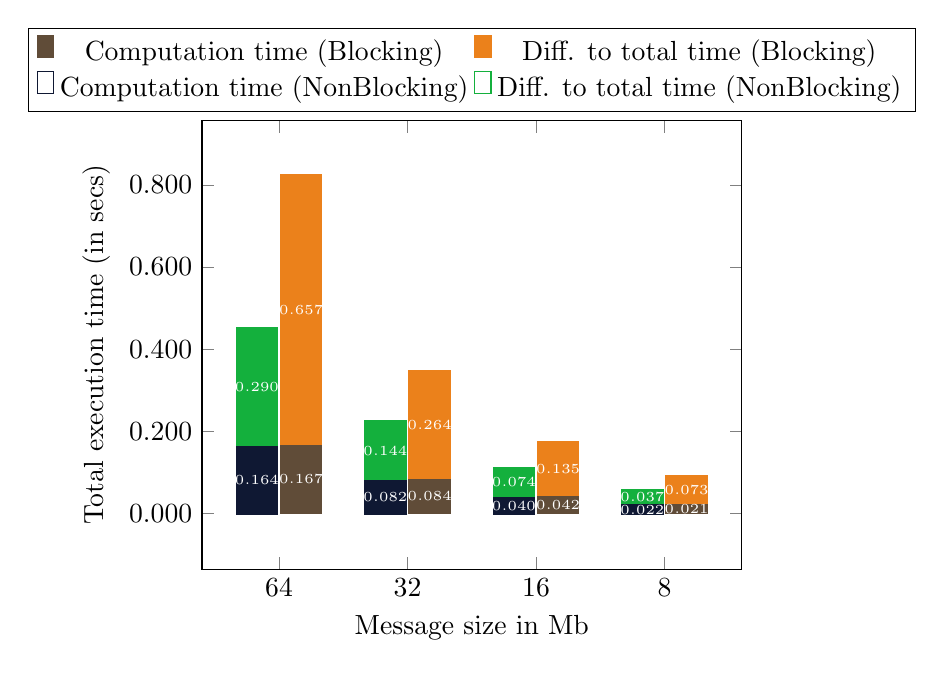
\begin{tikzpicture} [
            every axis/.style={ % add these settings to all the axis environments in the tikzpicture
                /pgf/number format/.cd, fixed, precision=3,1000 sep={}, zerofill,
                every node near coord/.append style={font=\tiny,},
                ybar stacked,
                %%x tick label style={rotate=45,anchor=east},
                symbolic x coords={
                    64, 32, 16, 8
                },
                enlargelimits=0.2,
                xtick=data,
                ymax=0.8,
                ylabel={Total execution time (in secs)},
                xlabel={Message size in Mb},
                ytick={0,0.2,0.4,0.6,0.8},
              bar width=15pt,
	          nodes near coords,
              },
        ]
\begin{axis}[
    ybar stacked,
    hide axis,
    bar shift=-8pt,
	bar width=15pt,
    legend style={at={(0.5,1.25)},
      anchor=north,legend columns=2},
    ]
\addplot[ybar,fill=mDarkTeal,draw=mDarkTeal,text=white] plot coordinates {(64,0.163979) (32,0.0819085) (16,0.0402079) (8,0.0222183)};
\label{nbct}
\addplot[ybar,fill=mLightGreen,draw=mLightGreen,text=white] plot coordinates {(64,0.289514) (32,0.144492) (16,0.0739917) (8,0.036825)};
\label{nbdt}
\end{axis}
\begin{axis}[
    bar shift=8pt,
    legend style={at={(0.5,1.02)},
      anchor=south,legend columns=2},
    ]
\addplot[ybar,fill=mDarkBrown,draw=mDarkBrown,text=white] plot coordinates {(64,0.167) (32,0.084) (16,.0417193) (8,0.0211096)};
\label{bct}
\addplot[ybar,fill=mLightBrown,draw=mLightBrown,text=white] plot coordinates {(64,0.657209) (32,0.26363) (16,0.134693) (8,0.07258)};
\label{bdt}
\addlegendentry{Computation time (Blocking)}
\addlegendentry{Diff. to total time (Blocking)}
\addlegendimage{/pgfplots/refstyle=bdt,color=mDarkTeal}
\addlegendentry{Computation time (NonBlocking)}
\addlegendimage{/pgfplots/refstyle=bdt,color=mLightGreen}
\addlegendentry{Diff. to total time (NonBlocking)}
\end{axis}
\end{tikzpicture}
    \end{center}
    \caption{Effect of message size on overlapping communication and computation (4 processors, OpenMPI 4, OpenFOAM 8); \scriptsize Benchmark inspired from \cite{Baruffa2020}}
\end{figure}
\end{frame}


\begin{frame}[fragile]{MPI send modes used in OpenFOAM code}
\begin{figure}
    \begin{center}
    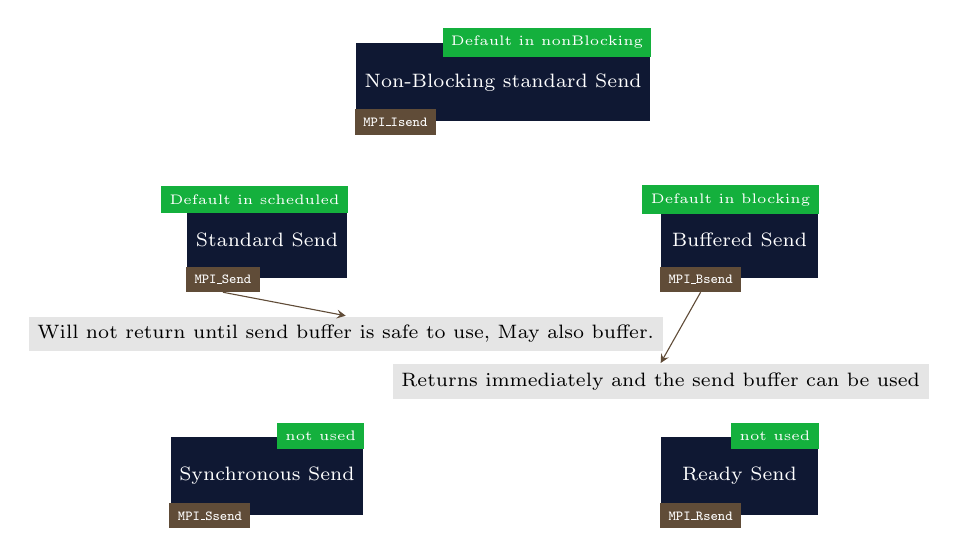
\begin{tikzpicture}
        \node[minimum height=1cm, minimum width=2cm,draw=white, text=white,fill=mDarkTeal] (m0) {\scriptsize Standard Send};
        \node[note] (n0) at (m0.north east)  {\tiny Default in scheduled};
        \node[lownote] (ln0) at (m0.south west)  {\tiny {\tt MPI\_Send}};
        \node[draw=white, fill=gray!20] (d0) at ($(m0)+(1cm,-1.2cm)$){\scriptsize
                Will not return until send buffer is safe to use,
                May also buffer.};
        \draw[-stealth, draw=mDarkBrown] (ln0.south) -- (d0.north);

        \pause
        \node[minimum height=1cm, minimum width=2cm,draw=white, text=white,fill=mDarkTeal] (m1) at ($(m0)+(6cm,0)$) {\scriptsize Buffered Send};
        \node[note] (n1) at (m1.north east)  {\tiny Default in blocking};
        \node[lownote] (ln1) at (m1.south west)  {\tiny {\tt MPI\_Bsend}};
        \node[draw=white, fill=gray!20] (d1) at ($(m1)+(-1cm,-1.8cm)$){\scriptsize
                Returns immediately and the send buffer can be used};
        \draw[-stealth, draw=mDarkBrown] (ln1.south) -- (d1.north);

        \pause
        \node[minimum height=1cm, minimum width=2cm,draw=white, text=white,fill=mDarkTeal] (m5) at ($(m0)+(3cm,2cm)$) {\scriptsize Non-Blocking standard Send};
        \node[note] (n5) at (m5.north east)  {\tiny Default in nonBlocking};
        \node[lownote] (ln5) at (m5.south west)  {\tiny {\tt MPI\_Isend}};

        \pause
        \node[minimum height=1cm, minimum width=2cm,draw=white, text=white,fill=mDarkTeal] (m2) at ($(m0)+(0,-3cm)$) {\scriptsize Synchronous Send};
        \node[note] (n2) at (m2.north east)  {\tiny not used};
        \node[lownote] (ln2) at (m2.south west)  {\tiny {\tt MPI\_Ssend}};
        \node[minimum height=1cm, minimum width=2cm,draw=white, text=white,fill=mDarkTeal] (m3) at ($(m1)+(0,-3cm)$) {\scriptsize Ready Send};
        \node[note] (n3) at (m3.north east)  {\tiny not used};
        \node[lownote] (ln3) at (m3.south west)  {\tiny {\tt MPI\_Rsend}};

    \end{tikzpicture}
    \end{center}
\end{figure}
\end{frame}

\section{Collective communication}

\begin{frame}[fragile]{Collective comms}
    When Two or more processes talk to each other.
    \begin{itemize}
        \item {\bf All processes} call the same function with the same set of arguments. 
        \item Although MPI-2 has non-blocking collective communications, OpenFOAM uses only the blocking variants.
        \item NOT a simple wrapper around P2P comms.
        \item OpenFOAM puts their interface in {\bf static public methods} of {\tt Pstream} class.
        \begin{itemize}
            \item Major differences in the API accross forks: (ESI and Foundation version) vs Foam Extend.
        \end{itemize}
    \end{itemize}
\end{frame}

\begin{frame}[fragile]{Collective comms}
    \begin{itemize}
        \item Most collective algorithms are $log(nProcs)$
        \item Gather (all-to-one), Scatter (one-to-all), All-to-All variants of all-to-one ones.
        \item OpenFOAM does not use all-to-one "reduce". What OpenFOAM calls a "reduce" is Gather+Scatter.
        \item MPI has also a "Broadcast" and "Barrier" but these are not used in OpenFOAM.
    \end{itemize}
\end{frame}

\begin{frame}[fragile]{Collective comms: Gather (All-to-one)}
\begin{CodeEnvNoComment}[Check how something is distributed over processors]{cpp}{\scriptsize}
bool v = false;
if (Pstream::master()){ v = something(); } // <- must do on master
Pstream::gather(v, orOp<bool>());  // <- root process gathers
\end{CodeEnvNoComment}
\begin{figure}
    \begin{center}
    \begin{tikzpicture}
    \node[loris1, process] (p0) [label=above:{\scriptsize $P_0$}] {};
    \node[lownote,inner sep=0.5mm,fill=white,draw=white,text=white] (ln0) at (p0.south west)  {\tiny $v_0$};
    \node[lownote,inner sep=0.5mm,fill=mDarkTeal,draw=mDarkTeal] (ln0) at (p0.south west)  {\tiny \only<1>{$v_0$}\only<2>{$v_0$}};
    \node[loris2, process] (p1) at (6,0) [label=above:{\scriptsize $P_1$}] {};
    \node[lownote,inner sep=0.5mm,fill=white,draw=white,text=white] (ln1) at (p1.south west)  {\tiny $v_0 || v_1 || v_2$};
    \node[loris1, process] (p2) at (3,2) [label=above:{\scriptsize $P_2$}] {};
    \node[lownote,inner sep=0.5mm,fill=white,draw=white,text=white] (ln2) at (p2.south west)  {\tiny $v_0 || v_1 || v_2$};
    \node[lownote,inner sep=0.5mm] (ln2) at (p2.south west)  {\tiny \only<1>{$v_2$}\only<2>{$v_2$}};
    \uncover<2> {
        \node (c) at ($(p0)+(3,-1)$) {   };
        \draw[thick,draw=mDarkTeal,Tee Barb-] (p0) |- (c.west) node [near end,above, mDarkTeal] {\tt orOp()};
        \draw[thick,draw=mLightGreen,-Tee Barb] (c.east) -| (p1) node [near start,above,mLightGreen] {\tt orOp()};
        \draw[thick,draw=mDarkBrown,-Tee Barb] (c.north) -- (p2) node [midway,above,mDarkBrown,rotate=90] {\tt orOp()};

        %\node[node, image] (x_src_i) [right=of y_src_i, label=below:$\phi_j$] { };
        \node (s1) at (3,-1) [circular sector,circular sector angle=120,fill=mLightGreen, minimum size=1mm, rotate=150, node distance=0,anchor=east] {};
        \node (s1) at (3,-1) [circular sector,circular sector angle=120,fill=mDarkTeal, minimum size=1mm, rotate=30,node distance=0,anchor=east] {};
        \node (s1) at (3,-1) [circular sector,circular sector angle=120,fill=mDarkBrown, minimum size=1mm, rotate=-90,node distance=0,anchor=east] {};
    }
    \node[lownote,inner sep=0.5mm,fill=mLightGreen,draw=mLightGreen] (ln1) at (p1.south west)  {\tiny \only<1>{$v_1$}\only<2>{$v_0 || v_1 || v_2$}};
    \end{tikzpicture}
    \end{center}
    \caption{An example OpenFOAM gather operation (More like a MPI-reduce)}
    \label{fig:}
\end{figure}
\end{frame}

\begin{frame}[fragile]{Collective comms: Gather (All-to-one)}
\begin{CodeEnvNoComment}[Check how something is distributed over processors (List-like)]{cpp}{\scriptsize}
List<bool> localLst(Pstream::nProcs(), false);
localLst[Pstream::myProcNo()] = something();
Pstream::gatherList(localLst); // <- root process gathers
\end{CodeEnvNoComment}
\begin{figure}
    \begin{center}
    \begin{tikzpicture}
    \node[loris1, process] (p0) [label=above:{\scriptsize $P_0$}] {};
    \node[lownote,inner sep=0.5mm,fill=mDarkTeal,draw=mDarkTeal] (ln0) at (p0.south west)  {\tiny $v_0$};
    \node[loris2, process] (p1) at (6,0) [label=above:{\scriptsize $P_1$}] {};
    \node[lownote,inner sep=0.5mm,fill=mLightGreen,draw=mLightGreen,anchor=center] (ln1) at (p1.south)  {\tiny $v_1$};
    \node[loris1, process] (p2) at (3,2) [label=above:{\scriptsize $P_2$}] {};
    \node[lownote,inner sep=0.5mm,anchor=east] (ln2) at (p2.south east)  {\tiny $v_2$};
    \uncover<2> {
        \node (c) at ($(p0)+(3,-1)$) {   };
        \draw[thick,draw=mDarkTeal,Tee Barb-] (p0) |- (c.west) node [near end,above, mDarkTeal] {};
        \draw[thick,draw=mLightGreen,-Tee Barb] (c.east) -| (p1) node [near start,above,mLightGreen] {};
        \draw[thick,draw=mDarkBrown,-Tee Barb] (c.north) -- (p2) node [midway,above,mDarkBrown,rotate=90] {};

        %\node[node, image] (x_src_i) [right=of y_src_i, label=below:$\phi_j$] { };
        \node (s1) at (3,-1) [circular sector,circular sector angle=120,fill=mLightGreen, minimum size=1mm, rotate=150, node distance=0,anchor=east] {};
        \node (s1) at (3,-1) [circular sector,circular sector angle=120,fill=mDarkTeal, minimum size=1mm, rotate=30,node distance=0,anchor=east] {};
        \node (s1) at (3,-1) [circular sector,circular sector angle=120,fill=mDarkBrown, minimum size=1mm, rotate=-90,node distance=0,anchor=east] {};
    }
    \node[lownote,inner sep=0.5mm,fill=white,draw=mDarkTeal,anchor=center] (ln0) at (p0.south)  {\tiny $v_0$};
    \node[lownote,inner sep=0.5mm,fill=white,draw=mDarkTeal,anchor=east] (ln0) at (p0.south east)  {\tiny $v_0$};
    \node[lownote,inner sep=0.5mm,fill=white,draw=mLightGreen,anchor=east] (ln1) at (p1.south east)  {\tiny $v_0$};
    \node[lownote,inner sep=0.5mm,fill=white,draw=mLightGreen,anchor=west] (ln1) at (p1.south west)  {\tiny $v_0$};
    \node[lownote,inner sep=0.5mm,fill=white,draw=mDarkBrown,anchor=center] (ln2) at (p2.south)  {\tiny $v_0$};
    \node[lownote,inner sep=0.5mm,fill=white,draw=mDarkBrown,anchor=west] (ln2) at (p2.south west)  {\tiny $v_0$};
    \uncover<2> {
    \node[lownote,inner sep=0.5mm,fill=mDarkBrown,draw=mDarkBrown,anchor=east] (ln1) at (p1.south east)  {\tiny $v_2$};
    \node[lownote,inner sep=0.5mm,fill=mDarkTeal,draw=mDarkTeal,anchor=west] (ln1) at (p1.south west)  {\tiny $v_0$};
    }
    \end{tikzpicture}
    \end{center}
    \caption{Example OpenFOAM gather operation on list items}
    \label{fig:}
\end{figure}
\end{frame}

\begin{frame}[fragile]{Collective comms: Scatter (One-to-all)}
\begin{CodeEnvNoComment}[Make processes know about something]{cpp}{\scriptsize}
bool v = false;
if (Pstream::master()){ v = something(); } // <- must do on master
Pstream::scatter(v);  // <- root process scatters
\end{CodeEnvNoComment}
\begin{figure}
    \begin{center}
    \begin{tikzpicture}
    \node[loris1, process] (p0) [label=above:{\scriptsize $P_0$}] {};
    \node[lownote,inner sep=0.5mm,fill=white,draw=white,text=white] (ln0) at (p0.south west)  {\tiny $v_0$};
    \node[lownote,inner sep=0.5mm,fill=mDarkTeal,draw=mDarkTeal] (ln0) at (p0.south west)  {\tiny \only<1>{$v_0$}\only<2>{$v_0$}};
    \node[loris2, process] (p1) at (6,0) [label=above:{\scriptsize $P_1$}] {};
    \node[lownote,inner sep=0.5mm,fill=white,draw=white,text=white] (ln1) at (p1.south west)  {\tiny $v_0 || v_1 || v_2$};
    \node[loris1, process] (p2) at (3,2) [label=above:{\scriptsize $P_2$}] {};
    \node[lownote,inner sep=0.5mm,fill=white,draw=white,text=white] (ln2) at (p2.south west)  {\tiny $v_0 || v_1 || v_2$};
    \node[lownote,inner sep=0.5mm] (ln2) at (p2.south west)  {\tiny \only<1>{$v_2$}\only<2>{$v_2$}};
    \uncover<2> {
        \node (c) at ($(p0)+(3,-1)$) {   };
        \draw[thick,draw=mDarkTeal,stealth-] (p0) |- (c.west);
        \draw[thick,draw=mLightGreen,-Tee Barb] (c.east) -| (p1);
        \draw[thick,draw=mDarkBrown,-stealth] (c.north) -- (p2);

        %\node[node, image] (x_src_i) [right=of y_src_i, label=below:$\phi_j$] { };
        \node (s1) at (3,-1) [circular sector,circular sector angle=120,fill=mLightGreen, minimum size=1mm, rotate=150, node distance=0,anchor=east] {};
        \node (s1) at (3,-1) [circular sector,circular sector angle=120,fill=mDarkTeal, minimum size=1mm, rotate=30,node distance=0,anchor=east] {};
        \node (s1) at (3,-1) [circular sector,circular sector angle=120,fill=mDarkBrown, minimum size=1mm, rotate=-90,node distance=0,anchor=east] {};
        \node[lownote,inner sep=0.5mm,fill=mLightGreen,draw=mLightGreen] (ln0) at (p0.south west)  {\tiny $v_1$};
        \node[lownote,inner sep=0.5mm,fill=mLightGreen,draw=mLightGreen] (ln2) at (p2.south west)  {\tiny $v_1$};
    }
    \node[lownote,inner sep=0.5mm,fill=mLightGreen,draw=mLightGreen] (ln1) at (p1.south west)  {\tiny \only<1>{$v_1$}\only<2>{$v_1$}};
    \end{tikzpicture}
    \end{center}
    \caption{An example OpenFOAM scatter operation (More like a MPI-Bcast)}
    \label{fig:}
\end{figure}
\end{frame}


\begin{frame}[fragile]{Collective comms: Scatter (One-to-all)}
\begin{CodeEnvNoComment}[Make processes know about something (List-like)]{cpp}{\scriptsize}
List<bool> localLst(Pstream::nProcs(), false);
if (Pstream::master()){ forAll(localLst, ei) { localLst[ei] = something(); } }
Pstream::scatterList(localLst); // <- root process scatters
\end{CodeEnvNoComment}
\begin{figure}
    \begin{center}
    \begin{tikzpicture}
    \node[loris1, process] (p0) [label=above:{\scriptsize $P_0$}] {};
    \node[lownote,inner sep=0.5mm,fill=white,draw=mDarkTeal] (ln0) at (p0.south west)  {\tiny $v_0$};
    \node[lownote,inner sep=0.5mm,fill=mDarkTeal,draw=mDarkTeal] (ln0) at (p0.south west)  {\tiny $v_0$};
    \node[loris2, process] (p1) at (6,0) [label=above:{\scriptsize $P_1$}] {};
    \node[lownote,inner sep=0.5mm,fill=mLightGreen,draw=mLightGreen,anchor=center] (ln1) at (p1.south)  {\tiny $v_1$};
    \node[loris1, process] (p2) at (3,2) [label=above:{\scriptsize $P_2$}] {};
    \node[lownote,inner sep=0.5mm,fill=white,draw=mDarkBrown,anchor=east] (ln2) at (p2.south east)  {\tiny $v_2$};
    \node[lownote,inner sep=0.5mm,fill=mDarkBrown,anchor=east] (ln2) at (p2.south east)  {\tiny $v_2$};
    \node[lownote,inner sep=0.5mm,fill=white,draw=mDarkTeal,anchor=center] (ln0) at (p0.south)  {\tiny $v_1$};
    \node[lownote,inner sep=0.5mm,fill=white,draw=mDarkTeal,anchor=east] (ln0) at (p0.south east)  {\tiny $v_2$};
    \node[lownote,inner sep=0.5mm,fill=white,draw=mDarkBrown,anchor=center] (ln2) at (p2.south)  {\tiny $v_1$};
    \node[lownote,inner sep=0.5mm,fill=white,draw=mDarkBrown,anchor=west] (ln2) at (p2.south west)  {\tiny $v_0$};
    \uncover<2> {
        \node (c) at ($(p0)+(3,-1)$) {   };
        \draw[thick,draw=mDarkTeal,Tee Barb-] (p0) |- (c.west) node [near end,above, mDarkTeal] {};
        \draw[thick,draw=mLightGreen,-Tee Barb] (c.east) -| (p1) node [near start,above,mLightGreen] {};
        \draw[thick,draw=mDarkBrown,-Tee Barb] (c.north) -- (p2) node [midway,above,mDarkBrown,rotate=90] {};

        %\node[node, image] (x_src_i) [right=of y_src_i, label=below:$\phi_j$] { };
        \node (s1) at (3,-1) [circular sector,circular sector angle=120,fill=mLightGreen, minimum size=1mm, rotate=150, node distance=0,anchor=east] {};
        \node (s1) at (3,-1) [circular sector,circular sector angle=120,fill=mDarkTeal, minimum size=1mm, rotate=30,node distance=0,anchor=east] {};
        \node (s1) at (3,-1) [circular sector,circular sector angle=120,fill=mDarkBrown, minimum size=1mm, rotate=-90,node distance=0,anchor=east] {};
    \node[lownote,inner sep=0.5mm,fill=mLightGreen,draw=mDarkTeal,anchor=center] (ln0) at (p0.south)  {\tiny $v_1$};
    \node[lownote,inner sep=0.5mm,fill=mLightGreen,draw=mDarkTeal,anchor=east] (ln0) at (p0.south east)  {\tiny $v_2$};
    \node[lownote,inner sep=0.5mm,fill=mLightGreen,draw=mDarkBrown,anchor=center] (ln2) at (p2.south)  {\tiny $v_1$};
    \node[lownote,inner sep=0.5mm,fill=mLightGreen,draw=mDarkBrown,anchor=west] (ln2) at (p2.south west)  {\tiny $v_0$};
    }
    \node[lownote,inner sep=0.5mm,fill=white,draw=mLightGreen,anchor=east] (ln1) at (p1.south east)  {\tiny $v_0$};
    \node[lownote,inner sep=0.5mm,fill=white,draw=mLightGreen,anchor=west] (ln1) at (p1.south west)  {\tiny $v_0$};
    \node[lownote,inner sep=0.5mm,fill=mLightGreen,draw=mLightGreen,anchor=east] (ln1) at (p1.south east)  {\tiny $v_2$};
    \node[lownote,inner sep=0.5mm,fill=mLightGreen,draw=mLightGreen,anchor=west] (ln1) at (p1.south west)  {\tiny $v_0$};
    \end{tikzpicture}
    \end{center}
    \caption{Example OpenFOAM scatter operation on list items}
    \label{fig:}
\end{figure}
\end{frame}

\begin{frame}[fragile]{Collective comms: Reduce (All-to-All)}
\begin{CodeEnvNoComment}[Do something with a var on all processors (eg. sum them up)]{cpp}{\scriptsize}
// Second arg: a binary operation function (functors); see ops.H
Foam::reduce(localVar, sumOp<decltype(localVar)>());
localVar = Foam::returnReduce(nonVoidCall(), sumOp<decltype(localVar)>());
\end{CodeEnvNoComment}
\begin{figure}
    \begin{center}
    \begin{tikzpicture}
    \node[loris1, process] (p0) [label=above:{\scriptsize $P_0$}] {};
    \node[lownote,inner sep=0.5mm,fill=white,draw=white,text=white] (ln0) at (p0.south west)  {\tiny $v_0+v_1+v_2$};
    \node[lownote,inner sep=0.5mm,fill=mDarkTeal,draw=mDarkTeal] (ln0) at (p0.south west)  {\tiny \only<1>{$v_0$}\only<2>{$v_0+v_1+v_2$}};
    \node[loris2, process] (p1) at (6,0) [label=above:{\scriptsize $P_1$}] {};
    \node[lownote,inner sep=0.5mm,fill=white,draw=white,text=white] (ln1) at (p1.south west)  {\tiny $v_0+v_1+v_2$};
    \node[lownote,inner sep=0.5mm,fill=mLightGreen,draw=mLightGreen] (ln1) at (p1.south west)  {\tiny \only<1>{$v_1$}\only<2>{$v_0+v_1+v_2$}};
    \node[loris1, process] (p2) at (3,2) [label=above:{\scriptsize $P_2$}] {};
    \node[lownote,inner sep=0.5mm,fill=white,draw=white,text=white] (ln2) at (p2.south west)  {\tiny $v_0+v_1+v_2$};
    \node[lownote,inner sep=0.5mm] (ln2) at (p2.south west)  {\tiny \only<1>{$v_2$}\only<2>{$v_0+v_1+v_2$}};
    \uncover<2> {
        \node (c) at ($(p0)+(3,-1)$) {   };
        \draw[thick,draw=mDarkTeal,Tee Barb-] (p0) |- (c.west) node [near end,above, mDarkTeal] {\tt sumOp()};
        \draw[thick,draw=mLightGreen,-Tee Barb] (c.east) -| (p1) node [near start,above,mLightGreen] {\tt sumOp()};
        \draw[thick,draw=mDarkBrown,-Tee Barb] (c.north) -- (p2) node [midway,above,mDarkBrown,rotate=90] {\tt sumOp()};

        %\node[node, image] (x_src_i) [right=of y_src_i, label=below:$\phi_j$] { };
        \node (s1) at (3,-1) [circular sector,circular sector angle=120,fill=mLightGreen, minimum size=1mm, rotate=150, node distance=0,anchor=east] {};
        \node (s1) at (3,-1) [circular sector,circular sector angle=120,fill=mDarkTeal, minimum size=1mm, rotate=30,node distance=0,anchor=east] {};
        \node (s1) at (3,-1) [circular sector,circular sector angle=120,fill=mDarkBrown, minimum size=1mm, rotate=-90,node distance=0,anchor=east] {};
    }
    \end{tikzpicture}
    \end{center}
    \caption{An example OpenFOAM reduce operation (MPI-Allreduce)}
    \label{fig:}
\end{figure}
\end{frame}

\againframe<3>{f1}

\begin{frame}[fragile]{Collective comms: Issues}
You can still fall for endless loops if you're not careful!
\begin{CodeEnvNoComment}[Infinite loops due to early returns]{cpp}{\scriptsize}
void refineMesh(fvMesh& mesh, const label& globalNCells)
{
  label currentNCells = 0;
  do
  {
    // Perform calculations on all processors
    currentNCells += addCells(mesh);
    // On some condition, a processor should not continue, and
    // returns control to the caller
    if (Pstream::myProcNo() == 1) return; // <-- oops, can't do this
    // !!! who's going to reduce this!
    reduce(currentNCells, sumOp<label>());
  } while (currentNCells < globalNCells);
  return;
}
\end{CodeEnvNoComment}
\end{frame}

\againframe<4>{f1}

\section{How do I send my own data?}

\begin{frame}[fragile]{A graph to hold neighboring processors}

Say we have something like this:

\begin{CodeEnvNoComment}[A directed graph of nodes]{cpp}{\scriptsize}
struct Edge {
    label destination = -1;
    scalar weight = 0.0;
};
using Graph = List<List<Edge>>;
// Try to push an edge from master to all procs
Edge ej;
if (Pstream::master())
{
    ej.destination = 16;
    ej.weight = 5.2;
}
\end{CodeEnvNoComment}

{\scriptsize Note: Edge does not have the requirements to be in a List yet}

\end{frame}

\begin{frame}[fragile]{A graph to hold neighboring processors}
First, does this compile?

\begin{CodeEnv}[Push an edge from master to All]{cpp}{\tiny \raggedright \alert{\bf error:} No match for {\tt operator<<(OPstream\&,Edge\&)}\\ \alert{\bf error:} No match for {\tt operator>>(IPstream\&,Edge\&)}}{\scriptsize}
Pstream::scatter(ej);
\end{CodeEnv}

So, Edges can't be communicated as MPI messages, fix it:
\begin{CodeEnvNoComment}[Stream Operators for Edge class]{cpp}{\scriptsize}
Ostream&  operator<<(Ostream& os, Edge& e) {
    os << e.destination << " " << e.weight;
    return os;
}
Istream&  operator>>(Istream& is, Edge& e) {
    is >> e.destination;
    is >> e.weight;
    return is;
}
\end{CodeEnvNoComment}
\end{frame}

\begin{frame}[fragile]{A graph to hold neighboring processors}
Try again:

\begin{CodeEnv}[Gathering info about graph nodes]{cpp}{\tiny Compiles, and works as expected}{\scriptsize}
Pstream::gatherList(g);
Pstream::scatterList(g);

// Check graph edges on all processes
Pout << g << endl;
\end{CodeEnv}


A Better way: Make Edge a child of one of the OpenFOAM classes
\begin{CodeEnvNoComment}[Better ways to define an Edge]{cpp}{\scriptsize}
struct Edge : public Tuple2<label, scalar> {};
// That's it, Edge is now fully MPI-ready
\end{CodeEnvNoComment}

\end{frame}

\section{Application examples \& advanced topics}

\newcommand{\highlight}[1]{\colorbox{mLightGreen!50}{$\displaystyle #1$}}

\begin{frame}[fragile]{Solving PDEs over decomposed domains (P2P comms)}
General Transport Equation for a physical transport property
$$
\partial_{t} \phi+\highlight{\nabla \cdot(\phi \mathbf{u})-\nabla \cdot(\Gamma \nabla \phi)}=S_{\phi}(\phi)
$$
Discretized form (Finite Volume notation)
$$
\llbracket \partial_{t}[\phi] \rrbracket+\highlight{\llbracket \nabla \cdot\left(F[\phi]_{f(F, S, \gamma)}\right) \rrbracket-\llbracket \nabla \cdot\left(\Gamma_{f} \nabla[\phi]\right) \rrbracket}=\llbracket S_{I}[\phi] \rrbracket .
$$

\begin{itemize}
    \item Receive neighbour values from neighbouring processor.
    \item Send face cell values from local domain to neighouring processor
    \item Interpolate to processor patch faces
\end{itemize}

\end{frame}


\begin{frame}[fragile]{Adaptive Mesh Refinement on polyhedral meshes}

    \begin{enumerate}
        \item Refine each processor's part of the mesh, but we need to keep the global cell count under a certain value: 
    \end{enumerate}
\begin{CodeEnvNoComment}[Reduce nAddCells or nTotalAddCells?]{cpp}{\scriptsize}
label ?\color{mDarkBrown!90}{nAddCells}? = 0;
label nIters = 0;
label ?\alert{nTotalAddCells}? = 0;
do
{
    ?\color{mDarkBrown!90}{nAddCells}? = 0;
    if (edgeBasedConsistency_)
    {
        ?\color{mDarkBrown!90}{nAddCells}? += edgeConsistentRefinement(refineCell);
    }
    ?\color{mDarkBrown!90}{nAddCells}? += faceConsistentRefinement(refineCell);
    reduce(?\color{mDarkBrown!90}{nAddCells}?, sumOp<label>());
    ++nIters;
    ?\alert{nTotalAddCells}? += ?\color{mDarkBrown!90}{nAddCells}?;
} while (?\color{mDarkBrown!90}{nAddCells}? > 0);
\end{CodeEnvNoComment}
\end{frame}

\begin{frame}[fragile]{Adaptive Mesh Refinement on polyhedral meshes}

    \begin{enumerate}\addtocounter{enumi}{1}
        \item To decide on whether to refine cells at processor boundaries, we need cell levels from the other side:
    \end{enumerate}
\begin{CodeEnvNoComment}[Reduce nAddCells or nTotalAddCells?]{cpp}{\scriptsize}
// Code extracted from Foam Extend 4.1
labelList ownLevel(nFaces - nInternalFaces);
forAll (ownLevel, i)
{
    const label& own = owner[i + nInternalFaces];
    ownLevel[i] = updateOwner();
}

// Swap boundary face lists (coupled boundary update)
syncTools::swapBoundaryFaceList(mesh_, ownLevel, false);

// Note: now the ownLevel list actually contains the neighbouring level
// (from the other side), use alias (reference) for clarity from now on
const labelList& neiLevel = ownLevel;
\end{CodeEnvNoComment}
\end{frame}

%\section*{Advanced topics}

\begin{frame}{Advanced topics}

    The need for Load Balancing in AMR settings

    \begin{itemize}
        \item AMR operations tend to unbalance cell count distribution accross processors
        \item Using Blocking comms means more idle process time
            \begin{itemize}
                \item Non-Blocking are not a solution.
                \item Spending some time on rebalancing the mesh is.
            \end{itemize}
        \item Naturally, load balancing itself involves parallel communication!
    \end{itemize}
\end{frame}

\begin{frame}{Licensing}

    This work is licensed under a
    \href{http://creativecommons.org/licenses/by-sa/4.0/}{Creative Commons
    Attribution-ShareAlike 4.0 International License}.

    Code snippets are licensed under a \href{http://www.gnu.org/licenses/gpl.txt}{GNU Public License}.

    \begin{center}\ccbysa \hspace{2mm} \textsuperscript{2022}\end{center}

\end{frame}

\begin{frame}[standout]
  Questions?
\end{frame}

\appendix

\begin{frame}[fragile]{Compile and link against MPI implementations}
Compiler wrappers are your best friends!
\begin{CodeEnv}[Grab correct compiler/linker flags]{bash}{\tiny-I/usr/lib/x86\_64-linux-gnu/openmpi/include/openmpi ...\\-pthread -L/usr/lib/x86\_64-linux-gnu/openmpi/lib ...}{\scriptsize}
mpic++ --showme:compiler
mpic++ --showme:linker
\end{CodeEnv}

OpenFOAM environment autmatically figures things out for you:
\begin{CodeEnvNoComment}[Typical Make/options file for the ESI fork]{bash}{\scriptsize}
include $(GENERAL_RULES)/mpi-rules
EXE_INC = $(PFLAGS) $(PINC) ...
LIB_LIBS = $(PLIBS) ...
\end{CodeEnvNoComment}
\end{frame}

\begin{frame}[fragile]{Miscellaneous}
    \begin{itemize}
        \item MPI standards: Blocking send can be used with a Non-blocking receive, and vice-versa
        \item But OpenFOAM wrapping makes it "non-trivial" to get it to work
    \end{itemize}
    \begin{itemize}
        \item You can still use MPI API directly, eg.  if you need one-sided communication.
    \end{itemize}
    \begin{itemize}
        \item Overlapping computation and communication for non-blocking calls is implemented on the MPI side, so,
        put your computations after the recieve call.
    \end{itemize}
\end{frame}


\begin{frame}[allowframebreaks]{Sources and further reading}
\printbibliography[heading=none]
\end{frame}


\end{document}
